
\begin{figure} \begin{center}
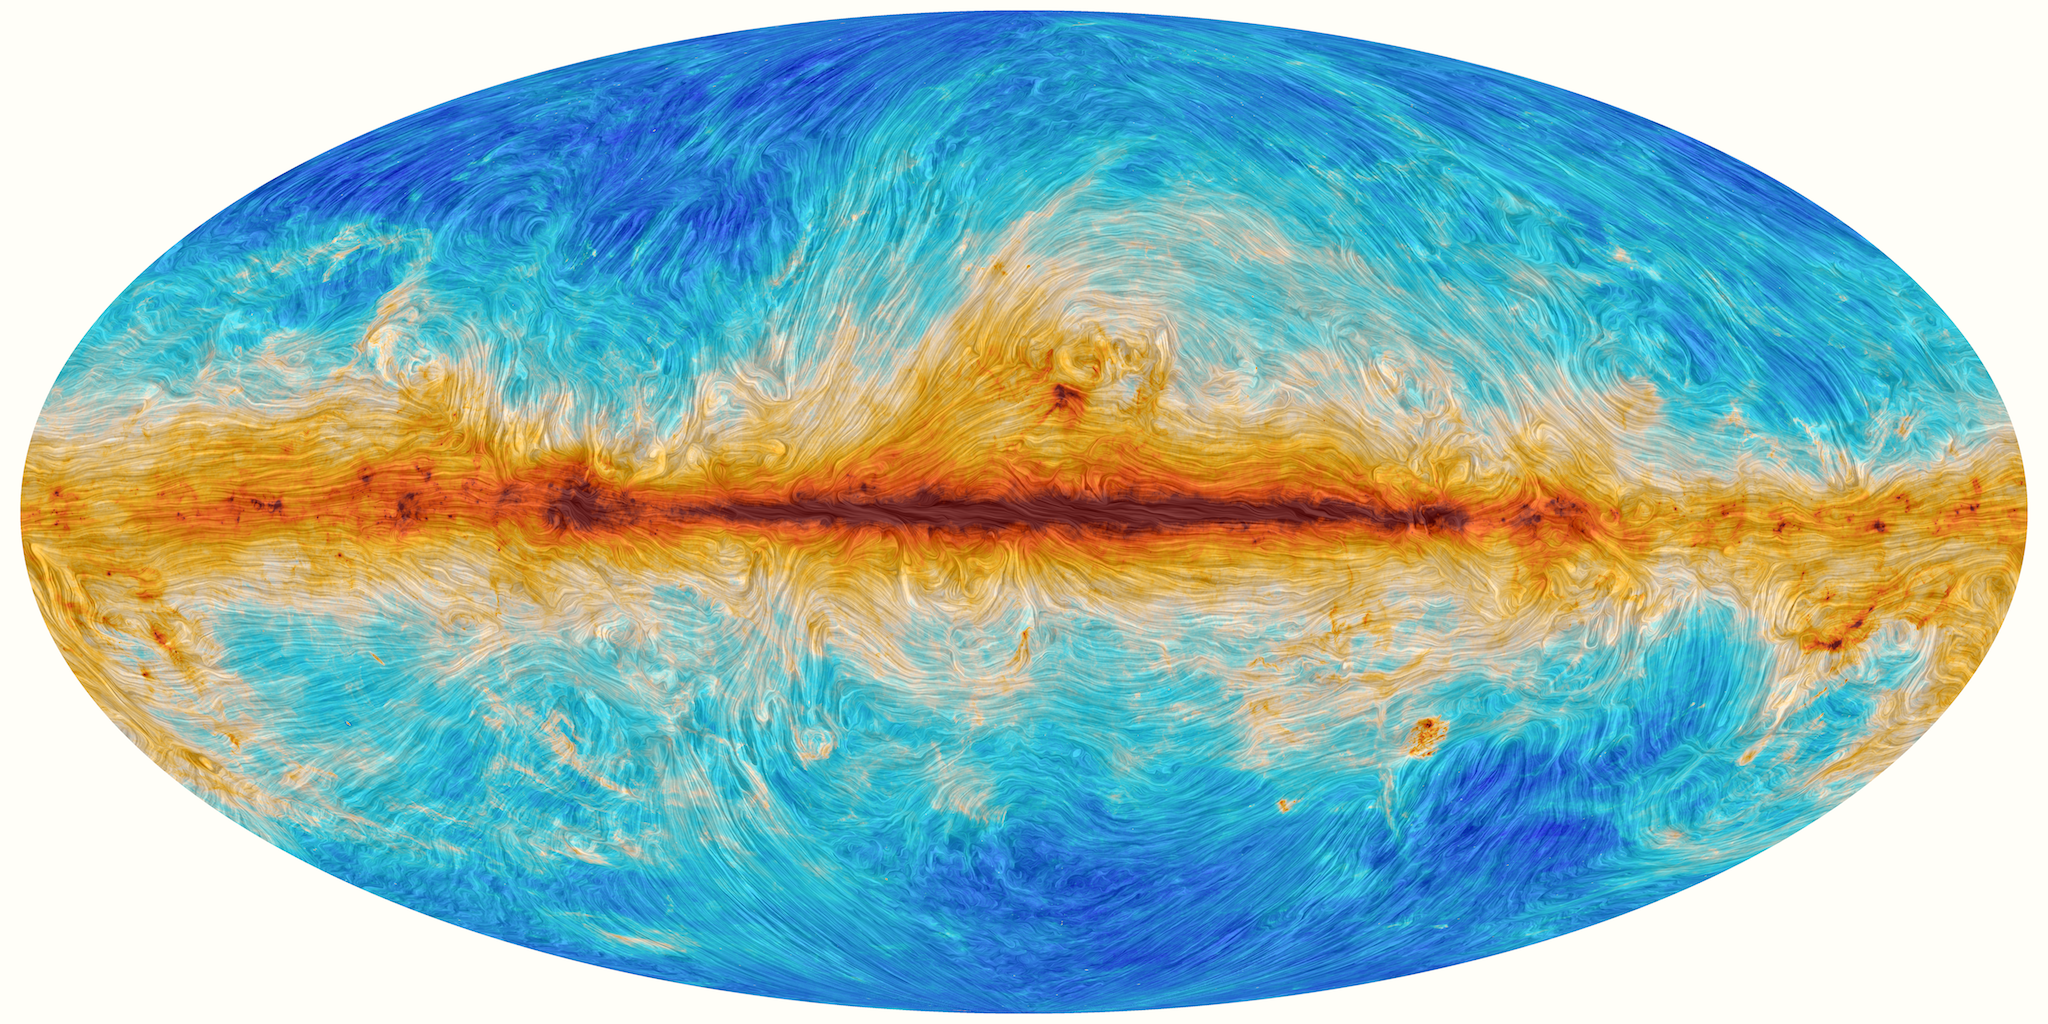
\includegraphics[width=0.9\textwidth]{figs/2015_353GHz_B-field.png}
\caption[ ]{The large scale magnetic field of the galaxy as seen by the Planck
satellite. The color field shows dust emission at 353GHz.  The image is smeared
along the direction of the magnetic field \citep{PlanckXIX15}.  The \nameCMB\
project aims to remove this signal from the CMB, while the \nameGalaxies\
project aims to understand its origin.}
\label{fig.planck} \end{center} \end{figure}
